\documentclass[12pt]{article}

\usepackage{import}
\usepackage{standalone}

\usepackage[top=4cm, right=2cm, bottom=2.7cm, left=2cm]{geometry}

\usepackage{wrapfig}
\usepackage{tabulary}
\usepackage{float}
\usepackage{pifont}
\usepackage{background}
\usepackage{tikz}


\pagestyle{empty}
\setlength{\parindent}{0pt}

\begin{document}
	\begin{minipage}{\textwidth}
		\section{Naar Beneden \hfill\small Bron: Bebras}
			Mevrouw Bever heeft een robot geplaatst bovenaan een doolhof. De robot daalt het doolhof af van het ene platform naar het andere eronder, totdat hij één van de vakken bereikt helemaal onderaan. Hiebij verplaatst hij zich altijd op dezelfde manier: hij verplaatst zich eerst naar rechts, en telkens wanneer hij een platform naar beneden valt, vertrekt hij opnieuw \textbf{in de omgekeerde richting}.
			
			De linker afbeelding hieronder toont het traject dat de robot zal volgen in het doolhof nr. 1. \\
	
			\begin{minipage}{0.49\linewidth}
				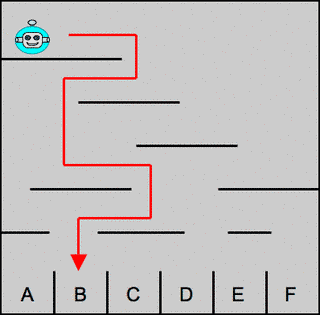
\includegraphics[width=\linewidth]{image1}
			\end{minipage} \hfill
			\begin{minipage}{0.49\linewidth}
				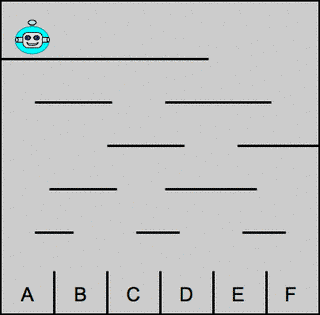
\includegraphics[width=\linewidth]{image2}
			\end{minipage}

	\end{minipage} \\ \\
	
\end{document}	